\chapter{Códigos}
%Aquí puedo incrustar tal cual los scripts del proyecto.
En este apéndice, describiremos los distintos scripts que podemos encontrar en las tarjetas Zybo con su explicación y código correspondiente.

Dicha descripción se hará siguiendo el orden que recorrerá el archivo recibido desde el dispositivo anterior hasta ser enviado al siguiente dispositivo.

Para comprobar el estado de todos los directorios, usaremos el comando \texttt{stat} para comprobar el estado de los directorios.

En el trabajo aquí mencionado se emula el desencriptado de un fichero, adición de información, cifrado, y envío del mismo a otro dispositivo\footnote{Para cambiar dicho comportamiento, solo tendremos que modificar los scritps que se encargan de automatizar el proceso.}. \textcolor{red}{Esto habría que cambiarlo puesto que ahora sí que tenemos el trabajo de Cristian.}

\newpage
\section{\texttt{Inicio.sh}}
\hypertarget{ScriptConexion}{}
El script se encarga de probar las conexiones de todos los dispositivos de la red para ver que están conectados al switch.

\subsection{Diagrama de flujo}
\begin{figure}[h]
	\centering
	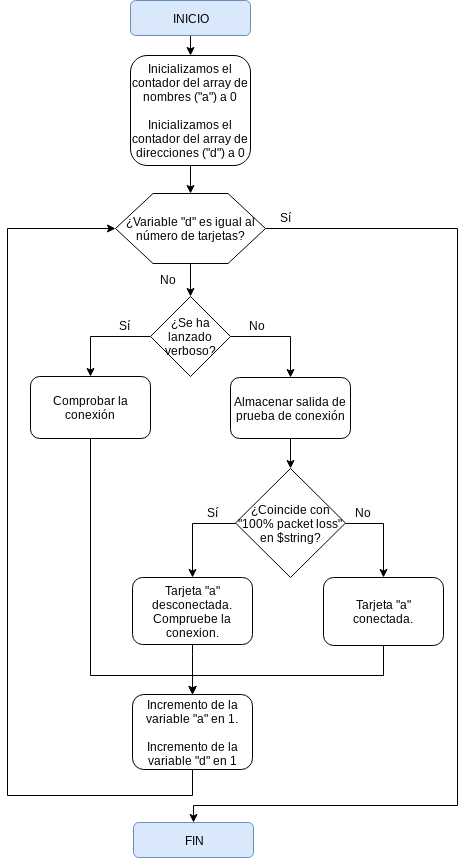
\includegraphics[scale=0.562]{Anexos/Anexo2/Test/Inicio.png}
	\caption{Diagrama de flujo de \texttt{Inicio.sh}}
	\label{Diagrama de flujo de Inicio.sh}
\end{figure}

\newpage
\subsection{Código}
\lstinputlisting[language=Bash]{Anexos/Anexo2/Test/Inicio.sh}
\begin{center}
	Código de \texttt{Inicio.sh} usando cuatro tarjetas como ejemplo.
\end{center}


\section{\texttt{Lanzador.sh}}
Este script se encarga de lanzar el script \texttt{Automatico.sh} mediante la herramienta cron\footnote{Para más información, ver el manual de crontab en este \href{https://linux.die.net/man/5/crontab}{\textcolor{blue}{enlace}}.} al inicio del sistema operativo Xillinux.

Para usarlo, debemos usar el siguiente comando:
\begin{center}
	\texttt{crontab -e}
\end{center}

Y, luego, añadir la regla que queramos que se ejecute al final del fichero. En nuestro caso es la siguiente:
\begin{center}
	\texttt{@reboot (cd \textasciitilde/ficheros; ./Lanzador.sh)}
\end{center}

Esto hará que la herramienta cron inicie este script al iniciar el sistema operativo Xillinux de las tarjetas Zybo.

\newpage
\subsection{Diagrama de flujo}
\begin{figure}[h]
	\centering
	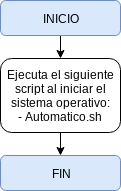
\includegraphics[scale=0.9]{Anexos/Anexo3/Diagramas/Lanzador.png}
	\caption{Diagrama de flujo de \texttt{Lanzador.sh}.}
	\label{Diagrama de flujo de Lanzador.sh}
\end{figure}

\subsection{Código}
\lstinputlisting[language=Bash]{Anexos/Anexo3/Scripts/Lanzador.sh}
\begin{center}
	Código de \texttt{Lanzador.sh}.
\end{center}


\newpage
\section{\texttt{Automatico.sh}}
Este script es el encargado de lanzar el resto de scripts periódicamente para que vayan comprobando los directorios correspondientes y se produzca la comunicación de forma automática.

%\newpage
\subsection{Diagrama de flujo}
\begin{figure}[h]
	\centering
	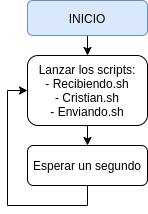
\includegraphics[scale=0.9]{Anexos/Anexo3/Diagramas/Automatico.png}
	\caption{Diagrama de flujo de \texttt{Automatico.sh}.}
	\label{Diagrama de flujo de Automatico.sh}
\end{figure}

\subsection{Código}
\lstinputlisting[language=Bash]{Anexos/Anexo3/Scripts/Automatico.sh}
\begin{center}
	Código de \texttt{Anexos/Anexo3/Automatico.sh}.
\end{center}


\newpage
\section{\texttt{Recibiendo.sh}}
Este script es el encargado de comprobar el estado del directorio \texttt{\textasciitilde/ficheros/recibir} y, si llega un archivo nuevo, enviarlo al directorio \texttt{\textasciitilde/ficheros/desencriptar}.

%\newpage
\subsection{Diagrama de flujo}
\begin{figure}[h]
	\centering
	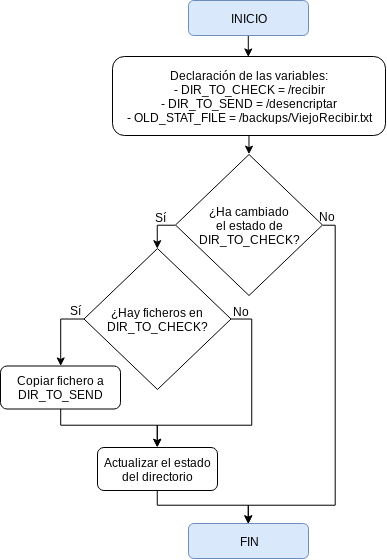
\includegraphics[scale=0.8]{Anexos/Anexo3/Diagramas/Recibiendo.png}
	\caption{Diagrama de flujo de \texttt{Recibiendo.sh}.}
	\label{Diagrama de flujo de Recibiendo.sh}
\end{figure}

\subsection{Código}
\lstinputlisting[language=Bash]{Anexos/Anexo3/Scripts/Recibiendo.sh}
\begin{center}
	Código de \texttt{Recibiendo.sh}.
\end{center}

\section{\texttt{Cristian.sh}}
\textcolor{red}{A este script le pondré el nombre \texttt{Encriptando.sh} seguramente, porque básicamente se encargará de eso (tanto encriptar como desencriptar), o, a unas malas, le pongo \texttt{Trabajando.sh}. También tengo la opción de hacer dos, uno que encripte y otro que desencripte, depende de como vea que funciona una vez que tenga las tarjetas. Así que, hasta que no tenga las tarjetas y me ponga a hacer las pruebas de verdad con todo (tanto lo de Gabri como lo de Cristian, esta parte queda un poco en el aire para perfeccionarla luego.).}

Este script es el encargado de emular el trabajo de nuestro compañero Cristian y realiza las siguientes tareas:
\begin{itemize}
	\item Gracias al crontab establecido, se encarga de comprobar periódicamente el estado del directorio \texttt{\textasciitilde/ficheros/desencriptar}.
	\item Mueve el archivo allí situado al directorio \texttt{\textasciitilde/ficheros/trabajar} (simulando el desencriptado del mismo).
	\item Una vez allí, añade un texto como el siguiente:
	\begin{center}
		\texttt{Archivo tratado en zyboX}
	\end{center}	
	Siendo zyboX el identificador de la tarjeta con la que estamos trabajando.
	\item Por último, envía el fichero al directorio \texttt{\textasciitilde/ficheros/enviar}.
\end{itemize}

\newpage
\subsection{Diagrama de flujo}
\begin{figure}[h]
	\centering
	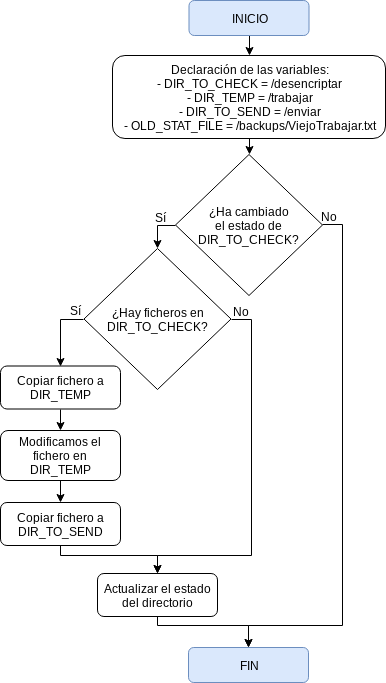
\includegraphics[scale=0.7]{Anexos/Anexo3/Diagramas/Cristian.png}
	\caption{Diagrama de flujo de \texttt{Cristian.sh}.}
	\label{Diagrama de flujo de Cristian.sh}
\end{figure}

\newpage
\subsection{Código}
\lstinputlisting[language=Bash]{Anexos/Anexo3/Scripts/Cristian.sh}
\begin{center}
	Código de \texttt{Cristian.sh}.
\end{center}

\newpage
\section{\texttt{Enviando.sh}}
\hypertarget{ScriptEnviando}{}
Este script es el encargado de comprobar periódicamente el estado del directorio\\ \texttt{\textasciitilde/ficheros/enviar} y, cuando detecta un cambio, envía el archivo a la siguiente tarjeta, o, si ésta se encuentra desconectada, al ordenador central.

A la hora de comprobar si la siguiente tarjeta está conectada o no, se hace enviando un comando ping a la siguiente tarjeta, por lo que se nos presentarán dos posibles casos:
\begin{itemize}
	\item \textbf{Éxito:} La tarjeta está conectada y será allí donde se envíe el fichero.
	\item \textbf{Fracaso:} La tarjeta no está conectada y el fichero será enviado al ordenador central.
\end{itemize}

Para que podamos usar el comando ping desde este script, debemos darle permisos de ejecución en modo usuario de la siguiente forma:
\begin{enumerate}
	\item Entramos como super-usuario con el comando \texttt{su} y contraseña \texttt{zyboX} (siendo X el identificador de la tarjeta con la que estamos trabajando).
	\item A continuación, introducimos el siguiente comando:
	\begin{center}
		\texttt{chmod u+s /bin/ping}
	\end{center}
	Y con eso, quedaría activado el comando \texttt{ping} para poder usarlo desde este script.
\end{enumerate}

\newpage
\subsection{Diagrama de flujo}
\begin{figure}[h]
	\centering
	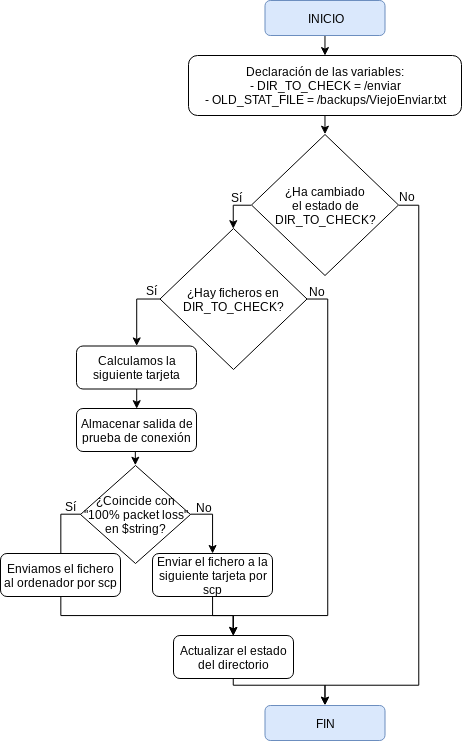
\includegraphics[scale=0.65]{Anexos/Anexo3/Diagramas/Enviando.png}
	\caption{Diagrama de flujo de \texttt{Diagramas/Enviando.sh}.}
	\label{Diagrama de flujo de Enviando.sh}
\end{figure}

\newpage
\subsection{Código}
\lstinputlisting[language=Bash]{Anexos/Anexo3/Scripts/Enviando.sh}
\begin{center}
	Código de \texttt{Enviando.sh}.
\end{center}


\section{\texttt{Borrar.sh}}
Este script se encarga de borrar el contenido de los directorios \texttt{\textasciitilde/ficheros/recibir},\\ \texttt{\textasciitilde/ficheros/desencriptar}, \texttt{\textasciitilde/ficheros/trabajar} y \texttt{\textasciitilde/ficheros/enviar} de las tarjetas Zybo.

Para ejecutarlo solo debemos usar el siguiente comando en el directorio \texttt{\textasciitilde/ficheros} de las tarjetas Zybo:
\begin{center}
	\texttt{./Borrar.sh}
\end{center}

\subsection{Diagrama de flujo}
\begin{figure}[h]
	\centering
	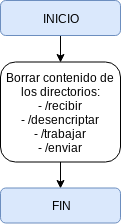
\includegraphics[scale=0.9]{Anexos/Anexo3/Diagramas/Borrar.png}
	\caption{Diagrama de flujo de \texttt{Borrar.sh}.}
	\label{Diagrama de flujo de Borrar.sh}
\end{figure}

%\newpage
\subsection{Código}
\lstinputlisting[language=Bash]{Anexos/Anexo3/Scripts/Borrar.sh}
\begin{center}
	Código de \texttt{Borrar.sh}.
\end{center}